\documentclass{article}

\usepackage[version=3]{mhchem}
\usepackage[greek,english]{babel}
\usepackage{booktabs}
\usepackage{gensymb}
\usepackage{graphicx}
\usepackage[hidelinks]{hyperref}
\usepackage{fixltx2e}
\usepackage{titlesec}
\usepackage[normalem]{ulem}
\usepackage{parskip}
\usepackage{multirow}
\usepackage{fancyvrb}
\usepackage{color}
\usepackage{float}
\usepackage[super]{nth}
\usepackage{minted}

\titleformat*{\section}{\Large\bfseries}
\titleformat*{\subsection}{\bfseries}

\hypersetup{
  colorlinks   = true,
  urlcolor     = blue,
  linkcolor    = black,
  citecolor    = black
}

\definecolor{grey}{gray}{0.65}

\newfloat{listing}{thp}{lop}
\floatname{listing}{Listing}

\usemintedstyle{borland}

\setcounter{secnumdepth}{0}

\newcommand{\calpha}{C\textsubscript{\textgreek{a}}}
\newcommand{\ahelices}{\textgreek{a}-helices}
\newcommand{\bsheets}{\textgreek{b}-sheets}
\newcommand{\bbphi}{\ensuremath{\phi}}
\newcommand{\bbpsi}{\ensuremath{\psi}}
\newcommand{\bbomega}{\ensuremath{\omega}}
\newcommand{\module}[2]{\href{#2}{\texttt{#1}}}
\newcommand{\atomrec}{\texttt{ATOM} record}

\newenvironment{problems}
{\subsubsection{Before moving on...} \begin{enumerate}}
{\end{enumerate}}

\begin{document}

\title{Making Ramachandran Plots}
\author{2014 iPQB Bootcamp\\Summer Programming Project}
\date{}
\maketitle{}

\section{Introduction}

The purpose of this project is to help you learn Python by giving you a
challenging but relevant problem to practice on.  In this project,
you will write a
program that generates Ramachandran plots from PDB files.  Ramachandran plots 
show how backbone torsion angles are distributed in proteins.  Different 
features of proteins (namely \ahelices{} and \bsheets{}) occupy distinct 
regions in these plots.  For this reason, Ramachandran plots are commonly used 
both to validate experimental structures and to predict computational 
structures.

Hopefully, this project will require you to exercise three skills that are 
essential for scientific programming:

\begin{enumerate}
 \item Reading in data from a file.
 \item Manipulating that data numerically.
 \item Plotting your results.
\end{enumerate}

If you have any questions about this project or programming in general, send me 
an email at \href{mailto:kale.kundert@ucsf.edu}{kale.kundert@ucsf.edu}.

\section{What is a Ramachandran Plot?}

I'll explain exactly what a Ramachandran plot is below, but I'll begin by 
introducing some basic terminology.  This is necessarily a brief introduction, 
so feel free to email me for clarification if it's too fast.  First of all, 
proteins are composed of amino acid residues.  Figure~\ref{fig:three-residues} 
shows three residues from a larger protein.  A distinction is made between the 
backbone (blue) and the sidechains (red).  Every residue in the protein is 
connected through the backbone, which has a very regular pattern of atoms: 
\ce{N - C_{\textgreek{a}} - C - N - C_{\textgreek{a}} - C - \ldots} where the 
carbon that supports the sidechain is called \calpha{} to distinguish it from 
the one that doesn't.

\begin{figure}
 \centering
 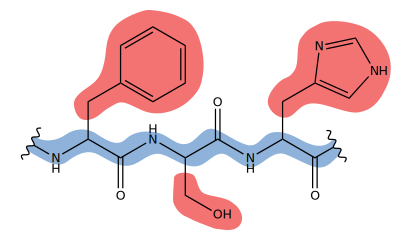
\includegraphics[width=0.65\textwidth]{three-residues}
 \caption{Three residues with the backbone and sidechains highlighted.}
 \label{fig:three-residues}
\end{figure}

Torsion angles are a convenient way to describe the geometry of the backbone.  
A torsion angle can be intuitively described
as the amount of twist around a bond.
To be more precise, consider four consecutive backbone atoms.  You always need 
four atoms to define a torsion angle.  Use the first three atoms to construct 
one plane and the last three atoms to construct another.  The angle between 
those two planes is the torsion angle, or the twist around the bond connecting 
the second and third atoms.  These angles are convenient way to describe 
geometry because they don't depend on the orientation of whole protein in 
Cartesian space.

For each residue in a protein, three backbone torsions are defined:

\begin{table}[h]
\centering
\begin{tabular}{cc}
\toprule
Torsion      & Backbone Atoms                                               \\
\midrule
$\omega{}_i$ & \ce{
C^{$i$-1}_{\textgreek{a}} - C^{$i$-1} - N^{$i$} - C^{$i$}_{\textgreek{a}}}  \\
$\phi{}_i$ & \ce{
C^{$i$-1} - N^{$i$} - C^{$i$}_{\textgreek{a}} - C^{$i$}}                    \\
$\psi{}_i$ & \ce{
N^{$i$} - C^{$i$}_{\textgreek{a}} - C^{$i$} - N^{$i+1$}}                    \\
\bottomrule
\end{tabular}
\caption{Backbone torsion angles.}
\label{tab:backbone-torsions}
\end{table}

A Ramachandran plot is a scatter plot showing the \bbphi{} and \bbpsi{} angles 
for each residue.  The \bbphi{} angles are plotted along the x-axis and the 
\bbpsi{} angles are plotted along the y-axis.  Each point is the $\phi_i, 
\psi_i$ pair for one residue.  The \bbomega{} angles are left out because they 
never deviate much from 180\degree.  

Figure~\ref{fig:example-plot} shows the Ramachandran plot for PDB ID: 1AXC, 
which is one of the structures I uploaded for you to use.  Note that there are 
two distinct clusters of points.  These represent two specific backbone 
conformations that are common in folded proteins: \ahelices{} (lower cluster) 
and \bsheets{} (upper cluster).  The ability to easily identify which residues 
are contributing to well-known, stable structural motifs is what makes 
Ramachandran plots useful for structural validation and prediction. 

\begin{figure}
 \centering
 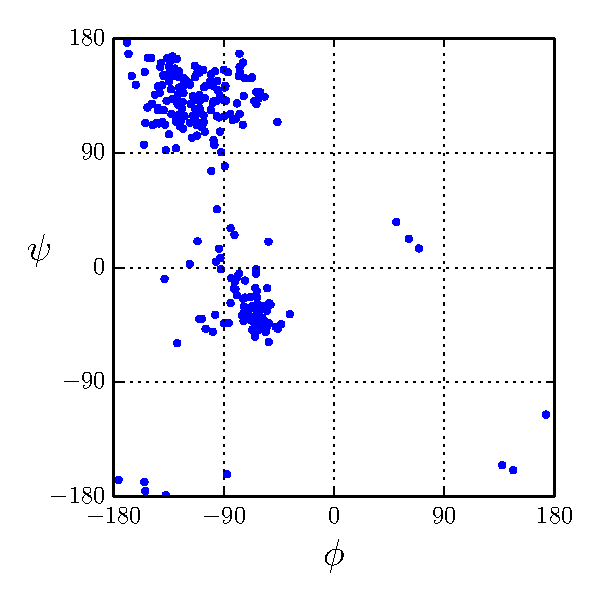
\includegraphics[width=0.48\textwidth]{example-plot}
 \caption{Ramachardran plot for PDB ID: 1AXC}
 \label{fig:example-plot}
\end{figure}

\section{What Do You Need to Do?}

Your task is to create a program written in Python that takes a PDB file 
(specified on the command line) as input and produces a Ramachandran plot as 
output.  Before starting you should work through an online tutorial.  There are 
lots of tutorials out there geared towards all different skill levels, but my 
favorite is \href{http://learnpythonthehardway.org/book}{Learn Python the Hard 
Way}.  It  includes  a 
\href{http://learnpythonthehardway.org/book/ex0.html}{section} on how to setup 
your computer to write and run Python programs.  Once you are ready to start 
the project, use the paragraphs below to guide how you write your  program.  
You can also download some example inputs from the
\href{http://bootcamp.ipqb.org/programming}{bootcamp website}.

\subsection{Part 1: Using Command Line Arguments}

Your program should accept the name of a PDB file as a command line argument.  
This will allow you to easily generate Ramachandran plots for different 
structures without having to change your script itself.  There are several ways 
to use command line arguments from python scripts.  If you're feeling 
overwhelmed and just want anything that works, look into 
\module{sys.argv}{http://learnpythonthehardway.org/book/ex13.html}.  If you're 
feeling more comfortable and want to learn how command line arguments are 
parsed in most modern python programs, look into 
\module{argparse}{https://docs.python.org/2.7/howto/argparse.html}.  And if you 
want to try an up-and-coming \texttt{argparse} alternative that beautifully 
marries parsing and documentation, look into 
\module{docopt}{https://github.com/docopt/docopt}.

\begin{problems}
\item Print out the name of a file specified on the command line.
\end{problems}

\subsection{Part 2: Reading PDB Files}

PDB files contain information about the 3D structure of proteins.  PDB stands 
for Protein Data Bank, which is online database of protein structures.  These  
files are regular text files (so you can view them with the same program you 
use to edit Python code) where each line contains different information about 
the structure.  The lines containing the information relevant to this project 
all begin with the keyword \texttt{ATOM}.  

\begin{listing}[h]
\centering
\begin{BVerbatim}[fontsize=\footnotesize,commandchars=\\\{\}]
\textcolor{grey}{         1         2         3         4         5         6         7         8}
\textcolor{grey}{12345678901234567890123456789012345678901234567890123456789012345678901234567890}
ATOM   2305  CA  ILE A 255      35.578   9.357   5.792  1.00 43.22           C  
\end{BVerbatim}
\caption{An example \atomrec{}.}
\label{list:pdb-example}
\end{listing}

Listing~\ref{list:pdb-example} shows an example \atomrec{}.  (The gray numbers 
aren't part of the record; they're just numbering the columns.)  Each 
\atomrec{} identifies a particular atom and specifies its coordinates.  
Different pieces of information about the atom are given at different offsets 
from the beginning of the line.  For example, the \nth{13} - \nth{16} 
characters of our example (\texttt{CA}) specify that the atom in question is a 
\calpha{}.  The \nth{18} - \nth{20} characters (\texttt{ILE}) specify that the 
atom is part of an isoleucine residue.
Table~\ref{tab:pdb-atom-record} describes the \atomrec{} fields that are most 
relevant to this project.  The complete 
\href{http://www.wwpdb.org/documentation/format33/v3.3.html}{PDB file format} 
is also available online if you're interested.

\begin{table}[h]
\centering
\begin{tabular}{r@{ - }rcll}
\toprule
\multicolumn{3}{l}{Columns} & Example         & Description                         \\
\midrule
 1 &  6 & & \texttt{ATOM}   & Fixed string identifying each line. \\
 7 & 11 & & \texttt{7507}   & Atom serial number.                 \\
13 & 16 & & \texttt{CA}     & Atom name.                          \\
18 & 20 & & \texttt{ILE}    & Residue name.                       \\
23 & 26 & & \texttt{255}    & Residue sequence number.            \\
31 & 38 & & \texttt{35.578} & X coordinate of atom.               \\
39 & 46 & & \texttt{9.357}  & Y coordinate of atom.               \\
47 & 54 & & \texttt{5.792}  & Z coordinate of atom.               \\
\bottomrule
\end{tabular}
\caption{Description of the fields in an \texttt{ATOM} record.}
\label{tab:pdb-atom-record}
\end{table}

Learning how to break big problems into smaller problems is an important skill 
for new programmers to practice.  This part of the project is a good place to 
do so because there are lots of ways to take small steps and get intermediate 
results when parsing a file.  The milestones listed below break down some of 
your first steps, but they may still be challenging.  If you get stuck, think 
about ways to break down these steps even further.

\begin{problems}
 \item Print out all the lines in a PDB specified on the command line.

 \item The same as above, but only print lines corresponding to backbone atoms 
  (i.e. lines where the atom name is either \texttt{N}, \texttt{CA}, or 
  \texttt{C}).

 \item The same as above, but only print the coordinates of the backbone atoms.

 \item Store the coordinates for each backbone atom in a tuple of three floats, 
  then store each of these tuples in a list.  Note that the coordinates have to 
  be converted to floats, because they are read in as strings.  As an example, 
  you should end up with a data structure that looks something like this: 

  \texttt{[(36.886, 53.177, 21.887), (38.323, 52.817, 21.996), ...]}

 \item To calculate each \bbphi{} and \bbpsi{} torsion, you need coordinates 
  for four atoms.  Table~\ref{tab:backbone-torsions} shows which coordinates 
  are needed for which torsion.  Write two loops: one that prints out the four 
  coordinates required for each \bbphi{} torsion and one that does the same for 
  each \bbpsi{} torsion.

\end{problems}

\subsection{Part 3: Calculating Torsion Angles}

Once you've read in Cartesian coordinates for all the backbone atoms, you'll 
need to calculate torsion angles.  You can find the algorithm for this 
calculation 
\href{http://math.stackexchange.com/questions/47059/how-do-i-calculate-a-dihedral-angle-given-cartesian-coordinates}{here}.  
Notice that this algorithm involves a healthy dose of vector arithmetic.  Since 
Python doesn't have built-in support for vector arithmetic, you'll have to 
write and test your own functions to perform the tasks outlined in 
Table~\ref{tab:vector-functions}.  Listing~\ref{lst:example-function} shows 
what one of these functions might look like.  Keep in mind that a vector is 
nothing more than a set of three coordinates, like the tuples we used above to 
store the backbone atom coordinates.  

\begin{table}[h]
\centering
\begin{tabular}{lll}
\toprule
Function                  & Example Input                & Example Output              \\
\midrule
Add two vectors           &
 \texttt{(1, 2, 3) (3, 4, 5)} & \texttt{(4, 6, 8)}          \\
Subtract two vectors      &
 \texttt{(1, 2, 3) (3, 4, 5)} & \texttt{(-2, -2, -2)}       \\
Normalize a vector        &
 \texttt{(1, 2, 3)}           & \texttt{(0.27, 0.53, 0.80)} \\
Calculate a dot product   &
 \texttt{(1, 2, 3) (3, 4, 5)} & \texttt{26}                 \\
Calculate a cross product &
 \texttt{(1, 2, 3) (3, 4, 5)} & \texttt{(-2, 4, -2)}        \\
\bottomrule
\end{tabular}
\caption{Vector arithmetic functions.}
\label{tab:vector-functions}
\end{table}

\begin{listing}[h]
 \inputminted{python}{example-function.py}
 \caption{Example addition function.}
 \label{lst:example-function}
\end{listing}

Once you have written these functions, use them to create another function that 
calculates a torsion angle using the above algorithm.  This function should 
take four vectors as input and return a single angle as output.  

Functions are a good way to reduce \emph{code duplication}, which is when the 
same code appears multiple times in the same program.  Inexperienced 
programmers tend to duplicate a lot of code because they copy-and-paste instead 
of writing functions.  This is a problem because it makes the code easy to 
break later on; you could change how the code works in one place and forget to 
update all the places it was copied.  It's better to write a single function 
and to call it from anywhere you need to, so you can change the function itself 
later on and be sure that the rest of your code stays up to date.  While you're 
working on this part of the project, be aware of code duplication and try to 
avoid it.  (For example, the add and subtract functions are quite similar.  Can 
you use one to write the other?)

If you are feeling comfortable with functions and you want to learn more about 
object-oriented programming, try writing a vector class.  Classes are useful 
when you want to associate a particular set of data with a particular set of 
functions.  Vectors make an ideal class, because the coordinates are clearly 
the data and the arithmetic helpers are clearly the functions.

If you are feeling comfortable with functions and classes, try performing these 
calculations using the 
\module{numpy}{http://wiki.scipy.org/Tentative_NumPy_Tutorial} vector math 
library.  This is a very important library for scientific programmers, because 
it really facilitates working with large arrays of data.  It also makes Python 
feel more like Matlab in some ways, which might be appealing to those with a 
Matlab background.  Once you get past the learning curve, you'll find that 
\texttt{numpy} makes this calculation much easier.

\begin{problems}
 \item Write and test all the functions described above.
 \item Create two lists: one that contains all the \bbphi{} torsions and one 
  that contains all the \bbpsi{} torsions.  This should build on the two loops 
  you wrote at the end of the previous section.
\end{problems}

\subsection{Part 4: Making Plots}

Use \module{matplotlib}{http://matplotlib.org/users/pyplot_tutorial.html} to 
generate your Ramachandran plot.  The documentation for \texttt{matplotlib} is 
so detailed that it's actually pretty hard to understand, but the tutorial 
linked above isn't bad.  If you get stuck, feel free to send me an email.

\pagebreak

\section{Future Directions}

If you found this project to be useful and you want to continue improving your 
scientific programming skills, you might try one or more of the extra 
challenges listed below.  The first is the easiest, the second is focused on 
handling lots of data, and the third is focused on Python as a general-purpose 
language.

\subsection{1. Make a residue-specific plot}

Glycine and proline have very distinctive Ramachandran plots.  Modify your 
program to either show just glycines, just prolines, or everything except 
glycine and proline.  There won't be enough glycines or prolines in a single 
structure to really show what these plots look like, so try combining this with 
the challenge below to really fill in your plots.  Also, you might find it 
interesting to ponder why glycine and proline have distinctive plots if you 
don't already know.

\subsection{2. Make a combined plot for 10,000 structures}

Working with lots of data is an important skill for scientific programmers.  
Toward that end, I uploaded a subset of the CATH database comprising 11,926 PDB 
files to the website.  Download this data and modify your program to create a 
single Ramachandran plot for all of it.  Experiment with ways to quickly 
process so many files and to clearly present so many data points.

\subsection{3. Automatically download PDB files}

One of the nice things about Python is that it's not just for scientific 
programming, so there are libraries for doing things like downloading files 
from the web.  The PDB in particular makes it very easy to 
\href{http://www.rcsb.org/pdb/software/rest.do#search}{automatically download 
structures}.  Modify your program to accept a PDB ID rather than an actual 
file, then download that structure from the PDB and use it to generate the 
plot.  The \module{requests}{http://docs.python-requests.org} library is a good 
place to start.

\end{document}
